
% spacing if needed
\newcommand{\postfig}{\vspace{-.35cm}}
\newcommand{\praecapt}{\vspace{-.2cm}}
\newcommand{\prevspace}{\vspace{-.4cm}}

% figure commands (easier to use)
\newcommand{\fig}[3]{
\begin{figure}[!t]
 \centering
\centerline{\includegraphics[width=#3,keepaspectratio=true]{#1}}%\praecapt
\caption{#2}\label{fig:#1}%\postfig
\end{figure}
}

\newcommand{\figheight}[3]{
\begin{figure}[!t]
 \centering
\centerline{\includegraphics[height=#3,keepaspectratio=true]{#1}}%\praecapt
\caption{#2}\label{fig:#1}%\postfig
\end{figure}
}

\newcommand{\fignaked}[3]{
 \centering
\centerline{\includegraphics[width=#3,keepaspectratio=true]{#1}}%\praecapt
\caption{#2}\label{fig:#1}%\postfig
}

\newcommand{\figb}[3]{
\begin{figure}[!b] 
%\vspace{-.3cm}
 \centering
\centerline{\includegraphics[width=#3,keepaspectratio=true]{#1}}%\praecapt
%\vspace{-.3cm}
\caption{#2}\label{fig:#1}%\postfig
\end{figure}
}

\newcommand{\figbheight}[3]{
\begin{figure}[!b] 
%\vspace{-.3cm}
 \centering
\centerline{\includegraphics[height=#3,keepaspectratio=true]{#1}}%\praecapt
%\vspace{-.3cm}
\caption{#2}\label{fig:#1}%\postfig
\end{figure}
}
\newcommand{\figbheightsmall}[3]{
\begin{figure}[!b] 
\vspace{-.3cm}
 \centering
\centerline{\includegraphics[height=#3,keepaspectratio=true]{#1}}%\praecapt
\vspace{-.3cm}
\caption{#2}\label{fig:#1}%\postfig
\end{figure}
}

\newcommand{\figfull}[3]{
\begin{figure*}[!t]
 \centering
\centerline{\includegraphics[width=#3,keepaspectratio=true]{#1}}%\praecapt
\caption{#2}\label{fig:#1}%\postfig
\end{figure*}
}



\newcommand{\RED}[1]{{\color{red}#1}}
\newcommand{\REM}[1]{{\color{blue}#1}}
\newcommand{\TODO}[1]{{\color{red}\footnote{\RED{#1}}}}
\newcommand{\lips}{\RED{\lipsum[1]}}

\newcommand{\smartos}{\textit{Smart}OS\xspace}
\newcommand{\moremcu}{\textit{more}MCU\xspace}

% some more fancy commands for abbreviation usage
\newcommand{\acd}[1]{\acl{#1} -- \acs{#1}\glsunset{#1}}
\newcommand{\acdp}[1]{\aclp{#1} -- \acsp{#1}\glsunset{#1}}
\newcommand{\acused}[1]{\glsunset{#1}}



\makeatletter
\newcommand{\monthyeardate}{%
  \DTMenglishmonthname{\@dtm@month} \@dtm@year
}
\makeatother



\newcommand{\summarydelimiter}{
\begin{center}
\medskip
  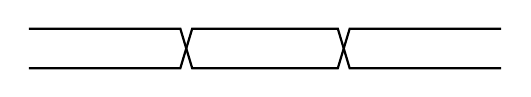
\begin{tikzpicture}[domain=0:7,scale=.5] 
  \draw[thick] (0,0) -- (3.85,0) -- (4.15,1) -- (7.85,1) -- (8.15,0) -- (12,0);
  \draw[thick] (0,1) -- (3.85,1) -- (4.15,0) -- (7.85,0) -- (8.15,1) -- (12,1);  
 
\end{tikzpicture}
\medskip
\end{center}
}

% referencing sections and chapters with their pages
\newcommand{\refp}[1]{\hyperref[#1]{\ref{#1}\hspace{.02cm}\textsuperscript{[p\pageref{#1}]}}}
\newcommand{\refpit}[1]{\hyperref[#1]{\ref{#1}\hspace{.08cm}\textsuperscript{[p\pageref{#1}]}}}
\newcommand{\refponly}[1]{\hyperref[#1]{\hspace{.02cm}\textsuperscript{[p\pageref{#1}]}}}
\newcommand{\see}{$\rightarrow$\xspace}

\newcommand{\hfillex}[1]{{%
      \unskip\nobreak\hfil\penalty50
      \hskip2em\hbox{}\nobreak\hfil{#1}%
      \parfillskip=0pt \finalhyphendemerits=0 \par}}

% backrefing in the bibliography
\renewcommand*{\backrefsep}{],~[p}
\renewcommand*{\backreftwosep}{],~[p}
\renewcommand*{\backreflastsep}{],~[p}
\renewcommand*{\backrefalt}[4]{\hfillex{\textsuperscript{\see~[p#2]}}}


\renewcommand*{\lstlistlistingname}{List of Listings}

% item counters in itemize environments
\newcounter{countitems}
\newcounter{nextitemizecount}
\newcommand{\setupcountitems}{%
  \stepcounter{nextitemizecount}%
  \setcounter{countitems}{0}%
  \preto\item{\stepcounter{countitems}}%
}
\makeatletter
\newcommand{\computecountitems}{%
  \edef\@currentlabel{\number\c@countitems}%
  \label{countitems@\number\numexpr\value{nextitemizecount}-1\relax}%
}
\newcommand{\nextitemizecount}{%
  \getrefnumber{countitems@\number\c@nextitemizecount}%
}
\makeatother
\AtBeginEnvironment{itemize}{\setupcountitems}
\AtEndEnvironment{itemize}{\computecountitems}


% Added for PlumeFit
\newcommand{\plumefit}{PlumeFit}
\usepackage{amsthm}
\newtheoremstyle{annahmenstil}%
  {\topsep}                    % Abstand oberhalb
  {\topsep}                    % Abstand unterhalb
  {\normalfont}                % Schrift des Körpers (aufrecht statt kursiv)
  {0pt}                        % Einzug der ersten Zeile
  {\bfseries}                  % Schrift des Kopfes
  {:}                          % Satzzeichen nach dem Kopf
  {\newline}                   % Abstand Kopf → Text; \newline = Umbruch
  {}                           % Kopf-Spezifikation (leer = Standard)

\theoremstyle{annahmenstil}
\newtheorem{annahme}{Annahme}
\renewcommand{\theannahme}{A\arabic{annahme}}
\providecommand*{\annahmeautorefname}{Annahme}

